\section{Conception et architecture de la solution}

\section{Vue d’ensemble de l’architecture}

L'architecture globale du projet repose sur une approche moderne, modulaire et automatisée, intégrant les principes de l'Infrastructure as Code, du GitOps, de la conteneurisation et de l'observabilité. Elle a été conçue pour répondre aux exigences de performance, de sécurité, de scalabilité et de maintenabilité en s'appuyant sur plusieurs principes de l’état de l’art et bonnes pratiques du génie logiciel et de l’ingénierie des plateformes

\begin{figure}[H]
	\centering
	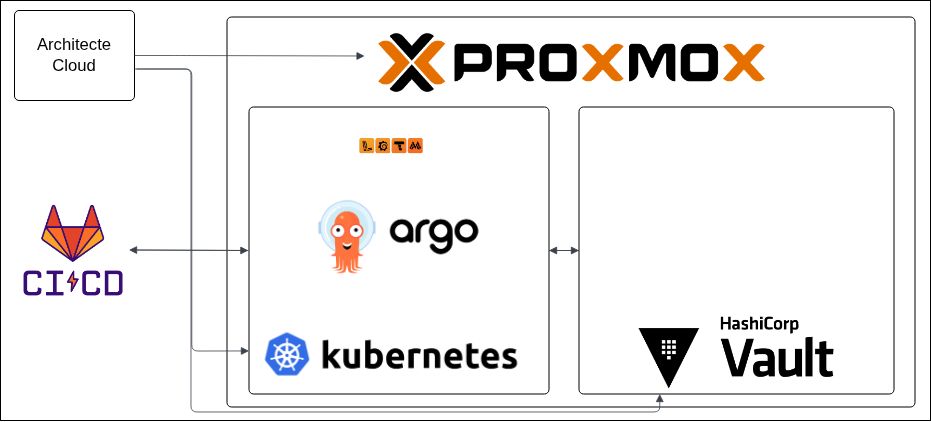
\includegraphics[width=0.9\textwidth]{figures/architecture-globale.png}
	\caption{Schéma d'architecture globale}
\end{figure}

\paragraph{\textbf{Infrastructure virtualisée et provisioning automatisé}}

L'infrastructure physique est virtualisée au moyen d'une plateforme Proxmox. La création des ressources a été entièrement automatisée via une démarche Infrastructure as Code.

\paragraph{\textbf{Infrastructure as Code avec Terraform}}

Terraform a permis de décrire et de provisionner l'ensemble des ressources suivantes de façon déclarative et reproductible :
\begin{itemize}
	\item Les machines virtuelles dédiées aux nœuds Kubernetes (masters et workers) et aux services utilitaires.
	\item Les réseaux virtuels, sous-réseaux et interfaces.
	\item Les volumes de stockage attachés aux instances.
	\item Les configurations initiales via cloud-init.
\end{itemize}

Les modules Terraform ont été organisés par domaines fonctionnels afin de favoriser leur réutilisation et leur évolutivité.

\begin{figure}[H]
	\centering
	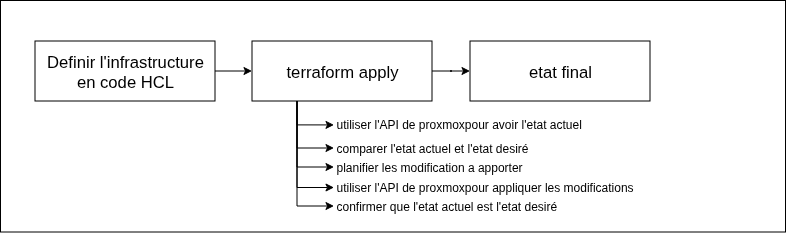
\includegraphics[width=0.8\textwidth]{figures/terraform-provisioning.png}
	\caption{Schéma du processus de provisioning automatisé avec Terraform}
\end{figure}

\paragraph{\textbf{Configuration automatisée avec Ansible}}

Après la création des ressources, Ansible assure la configuration des serveurs :
\begin{itemize}
	\item Installation et configuration du cluster Kubernetes.
	\item Déploiement des composants de monitoring et de sécurité.
	\item Configuration des services réseau et des paramètres système.
	\item Application des règles de sécurité renforcées.
\end{itemize}

Cette étape garantit l’homogénéité et la reproductibilité des environnements.

\begin{figure}[H]
	\centering
	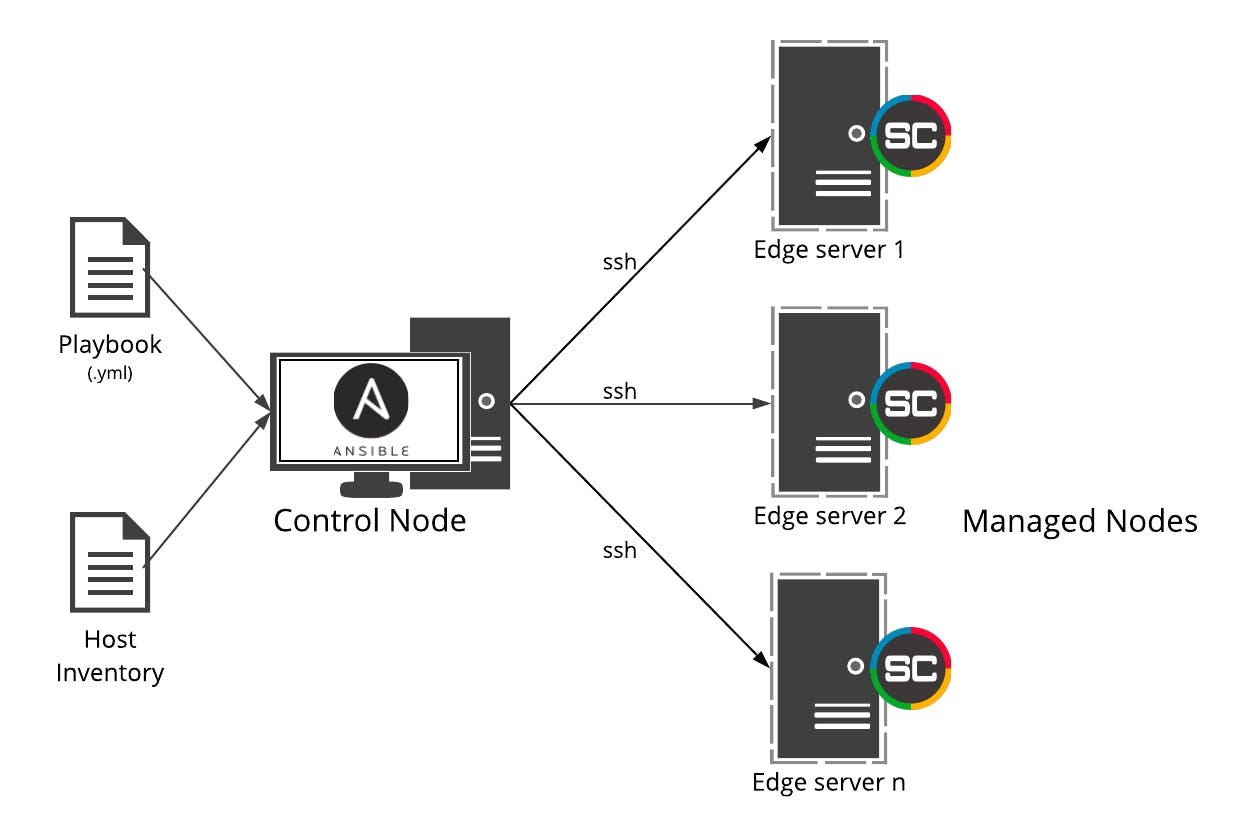
\includegraphics[width=0.8\textwidth]{figures/ansible-configuration.png}
	\caption{Processus d'automatisation de la configuration avec Ansible}
\end{figure}

\paragraph{\textbf{{Orchestration et déploiement applicatif}}

\paragraph{\textbf{Cluster Kubernetes}}

Kubernetes est le cœur de l’architecture d’orchestration. Il assure la gestion :
\begin{itemize}
	\item Du cycle de vie des conteneurs applicatifs.
	\item De l’équilibrage de charge et du scaling horizontal.
	\item De l’isolation des workloads.
\end{itemize}

\paragraph{\textbf{Déploiement GitOps avec Argo CD}}

Argo CD implémente une stratégie GitOps permettant :
\begin{itemize}
	\item Le déclenchement automatique des déploiements depuis un dépôt Git.
	\item La synchronisation continue des manifestes Kubernetes.
	\item La traçabilité complète des changements et la simplification des rollbacks.
\end{itemize}

\begin{figure}[H]
	\centering
	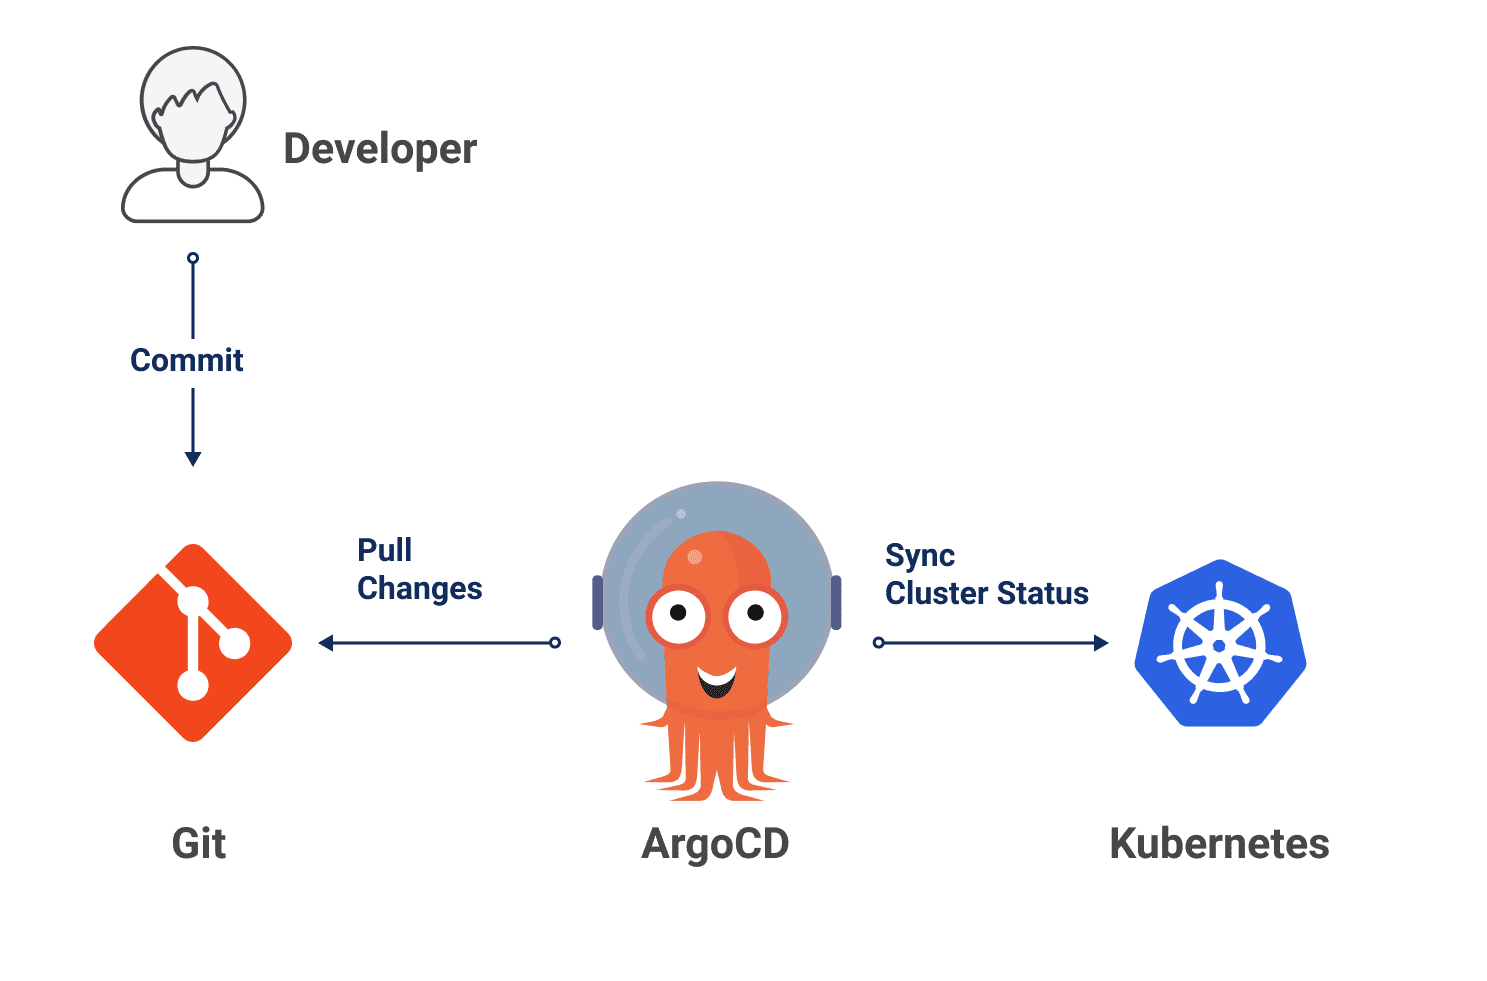
\includegraphics[width=0.9\textwidth]{figures/gitops-argo-cd.png}
	\caption{Flux GitOps des déploiements avec Argo CD}
\end{figure}

\paragraph{\textbf{Observabilité et monitoring}}

La supervision s'appuie sur un ensemble d’outils intégrés :

\begin{itemize}
	\item \textbf{Prometheus} pour la collecte des métriques et des alertes.
	\item \textbf{Grafana} pour la visualisation des indicateurs.
	\item \textbf{Loki} pour la centralisation des logs applicatifs et système.
	\item \textbf{Tempo} pour la gestion des traces distribuées.
\end{itemize}

Cette stack assure une observabilité complète et un diagnostic précis en cas d’incident.

\begin{figure}[H]
	\centering
	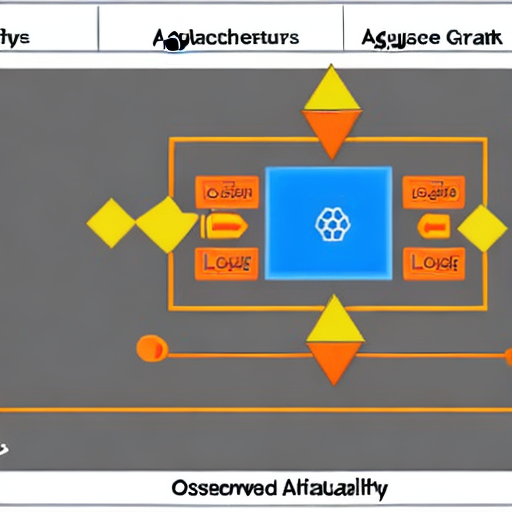
\includegraphics[width=0.85\textwidth]{figures/observabilite-stack.png}
	\caption{Architecture de la stack d'observabilité}
\end{figure}

\paragraph{\textbf{Stockage distribué et persistance des données}}

Le stockage persistant est assuré par Longhorn, qui fournit :
\begin{itemize}
	\item Des volumes répliqués tolérants aux pannes.
	\item Des snapshots automatisés et des fonctionnalités de restauration.
	\item Une intégration transparente avec Kubernetes.
\end{itemize}

\begin{figure} [H]
	\centering
	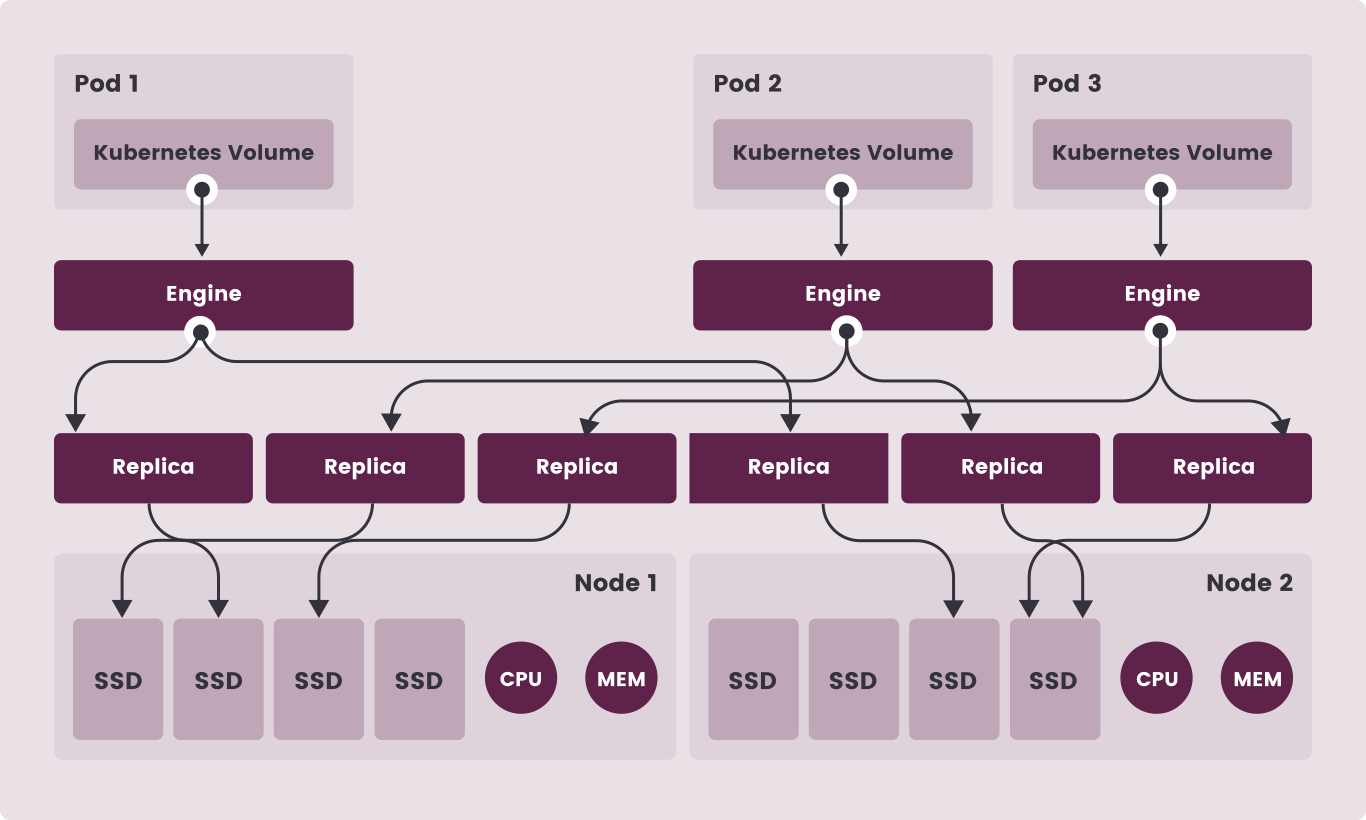
\includegraphics[width=.5\textwidth]{figures/how-longhorn-works.png}
	\caption{Stockage distribué avec Longhorn}
\end{figure}

\paragraph{\textbf{Gestion sécurisée des secrets}}

Vault joue le rôle de coffre-fort centralisé :
\begin{itemize}
	\item Stockage chiffré des mots de passe, certificats et tokens.
	\item Génération dynamique de secrets temporaires et rotation de secrets.
	\item Politiques d’accès granulaires pour limiter les droits.
\end{itemize}

\begin{figure}[H]
	\centering
	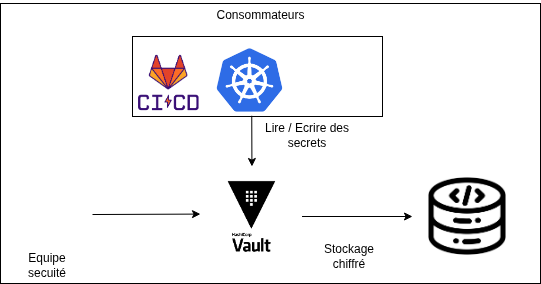
\includegraphics[width=0.8\textwidth]{figures/vault-gestion-secrets.png}
	\caption{Flux de gestion sécurisée des secrets avec Vault}
\end{figure}

\paragraph{\textbf{Sécurité réseau et accès administratifs}}

La sécurité périmétrique est confiée à un pare-feu pfSense :
\begin{itemize}
	\item Contrôle des flux entrants et sortants via des règles spécifiques.
	\item Mise en place d’un VPN pour les accès administratifs.
	\item Surveillance active des connexions.
\end{itemize}

\begin{figure}[H]
	\centering
	\begin{tikzpicture}[
			node distance=2cm,
			box/.style={draw, rectangle, minimum width=3cm, minimum height=1cm, align=center},
			vm/.style={draw, rectangle, minimum width=2cm, minimum height=0.8cm, align=center}
		]
		% Nodes
		\node[box] (internet) {Internet};
		\node[box, below of=internet] (proxmox) {Proxmox Hyperviseur};
		\node[box, below of=proxmox] (pfsense) {VM pfSense \\ (Pare-feu / Routeur)};
		\node[box, below of=pfsense] (switch) {Réseau LAN Interne};
		\node[vm, left=1.5cm of switch] (vm1) {VM1};
		\node[vm, right=1.5cm of switch] (vm2) {VM2};
		% Arrows
		\draw[->] (internet) -- (proxmox);
		\draw[->] (proxmox) -- (pfsense);
		\draw[->] (pfsense) -- (switch);
		\draw[->] (switch) -- (vm1);
		\draw[->] (switch) -- (vm2);
	\end{tikzpicture}
	\caption{Architecture de sécurité réseau avec pfSense}
\end{figure}

\paragraph{\textbf{Services internes pour le cycle de vie applicatif}}

Pour répondre aux besoins opérationnels des équipes, plusieurs services internes ont été déployés:
\begin{itemize}
	\item \textbf{GitLab} pour la gestion des dépôts, la CI/CD et la revue de code.
	\item \textbf{Harbor} comme registre privé de conteneurs.
	\item \textbf{YouTrack} pour le suivi des incidents et la gestion des tâches.
	\item \textbf{Nextcloud} pour le partage et l’archivage des documents.
\end{itemize}

Ces outils sont hébergés sur Kubernetes afin d’assurer leur haute disponibilité.

% Schéma services internes
\begin{figure}[H]
	\centering
	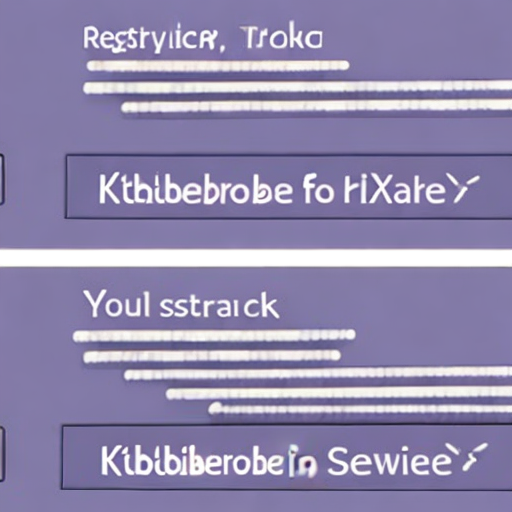
\includegraphics[width=0.85\textwidth]{figures/services-internes.png}
	\caption{Panorama des services internes}
\end{figure}

\paragraph{\textbf{Environnements de test et de production}}

\begin{itemize}
	\item Des environnements de \textbf{test} et de \textbf{staging} reprenant la même architecture que la production ont été mis en place afin de valider les développements et les mises à jour.
	\item Les environnements de \textbf{production} ont été configurés avec des sauvegardes automatiques et des mesures renforcées de sécurité et de supervision.
	\item Kustomize a ete utilisé pour garder une concistence et de gérer les variations de configuration entre les environnements, permettant de maintenir une base commune tout en adaptant les paramètres spécifiques (par exemple, les ressources allouées, les endpoints externes, etc.).
\end{itemize}

\paragraph{\textbf{Intégration et automatisation des déploiements}}

\textbf{GitLab CI/CD} joue un rôle central dans l'automatisation du cycle de vie applicatif. L’ensemble du pipeline est défini dans le fichier \texttt{.gitlab-ci.yml}, qui décrit les différentes étapes à exécuter pour chaque push, merge ou tag selon la configuration définie.

L’infrastructure GitLab repose sur plusieurs composants clés :
\begin{itemize}
	\item \textbf{.gitlab-ci.yml} : fichier principal décrivant les jobs et les stages du pipeline.
	\item \textbf{GitLab Runners} : exécutent les jobs dans des environnements isolés (VMs, containers...).
	\item \textbf{Variables GitLab} : utilisées pour stocker de manière sécurisée les credentials (tokens d’accès, clés API, identifiants, etc.), accessibles dans les jobs via des variables d’environnement.
	\item \textbf{Scripts et templates} : fichiers auxiliaires contenant les commandes d’automatisation (par exemple : \texttt{deploy.sh}, \texttt{test.sh}, \texttt{build.Dockerfile}).
\end{itemize}

\paragraph{\textbf{Structure générale d’un pipeline GitLab CI}}

Un pipeline CI/CD complet est généralement structuré autour des étapes suivantes :

\begin{itemize}
	\item \textbf{Validation}
	\item Formatage du code (ex : \texttt{black}, \texttt{prettier}, \texttt{clang-format}).
	\item Tests unitaires et fonctionnels (ex : \texttt{pytest}, \texttt{Jest}, \texttt{JUnit}).
	\item Analyse de dépendances (\texttt{OWASP Dependency-Check}, \texttt{safety}).
	\item Analyse de sécurité des secrets (\texttt{truffleHog}, \texttt{git-secrets}).
	\item Linting et analyse statique (ex : \texttt{ESLint}, \texttt{pylint}, \texttt{SonarQube}).
\end{itemize}

\begin{itemize}
	\item \textbf{Build}
	      \begin{itemize}
		      \item Compilation de binaires ou de librairies.
		      \item Construction d’images Docker avec \texttt{Dockerfile}.
		      \item Intégration des modules ou plugins nécessaires.
	      \end{itemize}
	\item \textbf{Package}
	      \begin{itemize}
		      \item Génération des artefacts (archives, packages, images).
		      \item Génération automatique de changelogs (\texttt{git-chglog}, \texttt{conventional-changelog}).
		      \item Mise à jour du \texttt{README}, documentation ou métadonnées.
	      \end{itemize}
	\item \textbf{Release}
	      \begin{itemize}
		      \item Création d’une release GitLab avec description, tag, et artefacts associés.
		      \item Publication vers des registries (DockerHub, GitLab Container Registry, PyPI, Maven, etc.).
		      \item Possibilité de signature cryptographique des artefacts.
	      \end{itemize}
	\item \textbf{Deploy}
	      \begin{itemize}
		      \item Déploiement automatique vers les environnements cibles (dev, staging, prod).
		      \item Utilisation de \texttt{kubectl}, \texttt{helm}, ou ArgoCD pour interagir avec Kubernetes.
		      \item Authentification via credentials sécurisés définis comme \texttt{CI/CD variables}.
	      \end{itemize}
	\item \textbf{Notify}
	      \begin{itemize}
		      \item Envoi de notifications Slack, Discord, Rocket.Chat, email ou webhook.
		      \item Génération de rapports HTML ou PDF avec les résultats des tests et des déploiements.
		      \item Archivage des logs dans des systèmes de monitoring (ELK, Loki, etc.).
	      \end{itemize}
\end{itemize}

\paragraph{\textbf{Exemple de gestion des credentials}}
Les variables sensibles telles que les clés d’accès API, tokens d'acces aux depots et tokens de déploiement ou credentials Kubernetes sont définies dans l’interface GitLab CI/CD (\texttt{Settings > CI/CD > Variables}) et injectées dans les jobs via :
\begin{verbatim}
deploy:
script:
- echo "$KUBECONFIG_SECRET" > kubeconfig
- kubectl --kubeconfig=kubeconfig apply -f k8s/
\end{verbatim}

\paragraph{\textbf{Exemple de stage de release}}
\begin{verbatim}
release:
stage: release
script:
- echo "Generating release..."
- git tag v${CI_COMMIT_SHORT_SHA}
- git push origin v${CI_COMMIT_SHORT_SHA}
- curl --header "PRIVATE-TOKEN: $GITLAB_TOKEN"
--data "name=Release v${CI_COMMIT_SHORT_SHA}&tag_name=v${CI_COMMIT_SHORT_SHA}"
"https://gitlab.com/api/v4/projects/${CI_PROJECT_ID}/releases"
\end{verbatim}

\begin{figure}[H]
	\centering
	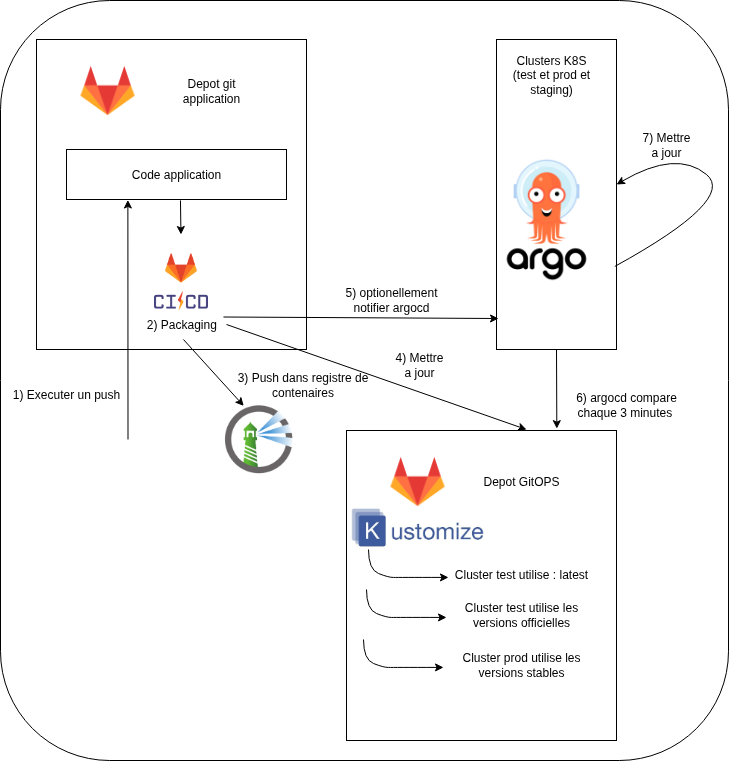
\includegraphics[width=0.85\textwidth]{figures/gitlab-ci.png}
	\caption{Processus d'intégration et de déploiement continu}
\end{figure}
